\section{Introduction and Literature Review} \label{introduction}
%This paper serves as a survey of weakly-hard constraints on real-time embedded systems. 

% Topic 1: importance of optimize embedded systems. 
\subsection{Embedded Systems}
In contrast to general-purpose computers such as personal computers which are designed to perform heterogeneous functions on one machine, embedded systems are designed to perform specific functions and are often components of larger systems. Embedded computers are the most prevalent type of computers in the current society with a wide range of applications including, but not limited to, control systems such as temperature control system in air conditioners, cruise control system in modern vehicles, and air-traffic control systems in airports. Because embedded systems are ubiquitous, it is important to optimize the design of embedded systems in terms of quality of service, energy consumption, security, robustness, and fault tolerance, etc, while guaranteeing the correctness of the systems. Because embedded systems are often parts of larger systems in which computation and communication resources are limited, it is important to optimize the resource usage for embedded systems. This paper studies a way to perform these optimization on the embedded systems designs by relaxing timing constraints imposed on them.

% Topic 2: hard, soft constraints are not enough.
\subsection{Real-time Constraints}
A characteristic of embedded systems is that they ought to satisfy real-time constraints. In the literature of real-time systems, a timing constraint for a task is defined as the deadline for each instance of the task. A constraint is \emph{hard} if the deadline has to be met, and \emph{soft} if the deadline can be missed occasionally. Correspondingly, a \emph{hard}  real-time model must meet all of its deadlines whereas a \emph{soft} real-time model can allow occasional deadline misses~\cite{liu2000real}.

However, the dichotomous classification between hard and soft constraints is not sufficient to formulate real-time embedded systems. On one hand, a soft real-time model cannot provide guarantees to performance and correctness requirements of some systems such as the stability requirement of some embedded controllers. On the other hand, a hard real-time model is too pessimistic for some systems that can tolerant bounded deadline misses. Given the limited computation and communication resources of embedded systems, it is a waste of resources to model such systems with hard real-time constraints. Moreover, it is possible that a tasks set that is not schedulable under the hard real-time model may become schedulable under a less-restricted real-time model. Therefore, we need to consider a timing constraint that is in the middle of hard and soft constraint. This paper studies \emph{weakly-hard} constraints, timing constraints that are weaker than hard constraints in that they allow deadline misses, but also harder than soft constraints in that the number of deadline misses within a time interval is bounded. 

% Topic 3: introduce weakly-hard constraints.
\subsection{Weakly Hard Constraints}
Weakly-hard constraints are constraints that allow deadline misses in a predictable manner. Weakly-hard systems are real-time systems whose distribution of met and missed deadlines is precisely bounded. A common model of weakly-hard systems is called (m-k) model, first proposed by Hamdaoui et al.~\cite{hamdaoui1995dynamic}. In the (m, k) model, there are at least m deadlines that are previously met in any consecutive sequence of k tasks (see Definition~\ref{def:meetany}). Later, Bernat et al.~\cite{bernat2001weakly} generalized the (m, k) model to four types of weakly-hard models that exhaust all possible real-life scenarios (see Section~\ref{model} for more details). Since then, works have been done in computing and verifying weakly-hard guarantees~\cite{bernat2001weakly, broster2002weakly, hammadeh2014extending,  sun2017weakly, ahrendts2018verifying, hammadeh2018weakly, huang2019formal, huang2020saw, pazzagliageneralized, choi2019job}, as well as applying the weakly-hard model to optimize the design and implementation of embedded systems~\cite{liang2019security, liang2020leveraging, maggio2020control}.

% Topic 4: computing weakly-hard guarantees.
\subsection{Weakly-hard Guarantees}
Various methods are proposed to compute the schedulability on weakly-hard systems. Response time analysis~\cite{joseph1986finding} is a common way to verify whether a task set is schedulable in the worst case. Broster et al.~\cite{broster2002weakly} utilized the technique of response time analysis to provide schedulability guarantees on weakly-hard models. However, the weakly-hard guarantee calculated by the response time analysis is pessimistic. Broster et al.~\cite{broster2002weakly} used simulation based experiments to show that many weakly hard constraints are not violated even at a much higher error rate than the limit calculated by the response time based schedulability analysis. Therefore, a better method to compute the weakly hard guarantees is needed. 

Typical Worst Case Analysis (TWCA) is a timing analysis technique that can provide a tighter bound than response time analysis for weakly hard models~\cite{quinton2012twca}. Hammadeh et al. utilized the TWCA method as well as an Integer Linear Programming (ILP) formulation to calculate the maximum occurrences of deadline misses for tasks with static priority scheduling policy~\cite{hammadeh2014extending}. Xu et al. improved the TWCA technique to calculate the deadline miss model by considering possible scenarios of sporadic overloads leading to occasional deadline misses~\cite{xu2015improve}. TWCA was then applied to calculating weakly-hard guarantees for systems with dependent task chain~\cite{hammadeh2017bound} and with weighted round-robin scheduling policy~\cite{hammadeh2018weakly}. Ahrendts et al. combined TWCA with Compositional Performance Analysis (CPA) to compute weakly-hard guarantees for distributed embedded systems with multiple resources~\cite{ahrendts2018verifying}.

There are methods other than TWCA that are used to calculate weakly-hard schedulability guarantees. Frehse et al.~\cite{frehse2014formal} proposed a model checking based hybrid technique for schedulability analysis on weakly-hard systems, but its scalability is limited by the computation complexity of model checking. Sun et al.~\cite{sun2017weakly} formulated the weakly-hard schedulability problem as Mixed Integer Linear Programming (MILP) problem for periodic tasks with static priorities without the knowledge of task offsets. However, this method's scalability is limited by the size of tasks because of the complexity of the MILP problem~\cite{sun2017weakly}. Pazzaglia et al. extended the scope of this method to include systems allowing jitters and resource sharing~\cite{pazzagliageneralized}, but this method still needs a significantly large amount of time to obtain an optimal solution to the large, complex MILP problem. Choi et al. improved the running time of the schedulability analysis with a new scheduling policy that classifies each task based on the number of deadlines that are previously met~\cite{choi2019job}. 

% Topic 5: verify guarantees
To show that the methods for computing weakly-hard constraints are sound, it is necessary to verify the safety and functional correctness of these weakly-hard guarantees on embedded systems. Duggirala et al. verified the safety of weakly hard guarantees on linear control systems by reducing the original verification problem to a software verification problem~\cite{duggirala2015analyzing}. Huang et al. extended the scope of the verification from linear systems proposed in~\cite{duggirala2015analyzing} to nonlinear system by adopting an over-approximation technique~\cite{huang2019formal}. Huang et al. also developed SAW, a tool that implements their verification method~\cite{huang2020saw}. 

% Topic 6: weakly hard model is useful for embedded systems.
\subsection{Usage of Weakly Hard Model}
Weakly hard models have various application to embedded systems including, but not limited to, intermittent computing systems, multi-rate distributed systems, image processing systems, and control systems. Intermittent computing systems are embedded systems whose computation may be occasionally suspended because of unreliable power supply, resulting in occasional deadline misses~\cite{talla2015powering, balsamo2016hibernus, colin2016chain, lucia2017intermittent}. The lack of stable power supply is possible for embedded systems because of the potential scarcity of resource for embedded systems. For example, embedded systems in an automatic vehicle that is crossing a desert are likely to not have continuous, stable power supply for embedded systems on the vehicle. An unstable power supply degenerates the quality of resources which are used by embedded systems. Therefore, design optimization is needed for embedded systems to overcome the challenges imposed by unstable power supply. 

Other than embedded systems with unreliable power supply, weakly hard model is useful for multi-rate distributed embedded systems that are sensitive to message losses. Distributed embedded systems with periodic scheduling policy are possible to have various rates for different components of the systems. For instance, in a distributed embedded control system, the sensor and the controller may operate at different rates. Specifically, bounded deadline misses will occur if the sensor has a higher operating frequency than the controller~\cite{li2015design}. Another type of embedded system that can have bounded deadline misses is an image processing system whose deadline misses are caused by the slow rate of human perception~\cite{yang2010adaboost}. Because these systems suffer from bounded deadline misses, the weakly hard model can provide flexible timing guarantees for these systems. 

\subsection{Control Systems}
This survey focuses on the application of weakly hard timing constraints on yet another type of embedded systems: control systems. As shown in Figure~\ref{fig:controller_model}, a control system consists of a physical plant and a controller which ensures certain behaviors of the physical plant. The controller consists of sensors which read data from the physical plant as input, electric computing units (ECUs) which compute control inputs, and actuators which perform operations on the physical plants indicated by the control inputs. We consider a common type of control systems in this paper: linear time-invariant control systems with feedback loops. This type of system is used to maintain the stability of the physical plant and ensure the states of the model of the physical plant to approach a referenced value. Therefore, scheduling policies ought to guarantee the stability and performance requirements of control systems. 

\begin{figure}[h!]
\caption{Control system model}
\centering
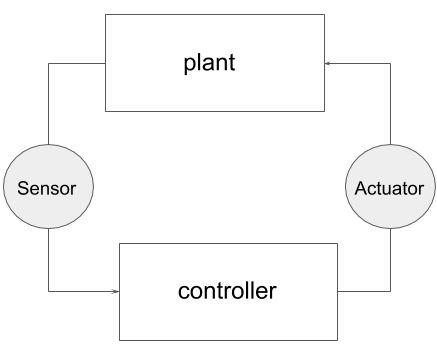
\includegraphics[width=0.5\textwidth]{controller_model}
\label{fig:controller_model}
\end{figure}

The weakly hard model can be a right fit for control systems because of the following intrinsic property of control systems: the stability and performance requirements of control systems can be satisfied despite occasional deadline misses, provided that no more than m deadlines misses can happen in any sequence of k deadlines, which is defined as the m-K model of weakly hard systems (see Definition~\ref{def:missany})~\cite{hamdaoui1995dynamic, ramanathan1999overload}. Goswami et al. formalized this property by proposing an analytical upper bound on deadline misses that allows distributed embedded control systems to maintain the stability as well as meet the performance requirements~\cite{goswami2014relax}. Control performance under deadline misses is also studied on an optimal linear quadratic regulator controller~\cite{horssen2016performance}. Linsenmayer et al. studies methods to design stable controllers given the weakly hard constraints~\cite{linsenmayer2017stabilization}. The degradation of performance caused by the deadline misses on weakly hard systems is studied as well. Pazzaglia et al. showed the impact of various deadline miss patterns on the control performance of the weakly hard system~\cite{pazzaglia2018beyond}. Lastly, Maggio et al.~\cite{maggio2020control} studied the stability of control systems with a different type of weakly hard models (m-K model, see Definition~\ref{def:missany} in Section~\ref{model}). Therefore, the reason why weakly hard model is applicable to control systems is formalized. 

% Topic 7: apply weakly-hard constraints to control systems. 
\subsection{Applying Weakly-hard Model to Control Systems}
Since reasons of applying weakly hard model to control systems were discussed, works have been done to exploit the application of weakly hard model on scheduling control tasks to enhance the security and robustness of the system. Liang et al. proposed a co-design approach to use weakly hard constraints on control tasks to improve systems' capability for hosting security monitoring tasks, thus enhancing the security of the system designs~\cite{liang2019security}. Liang et al. derived the weakly hard constraints on control tasks that satisfy the stability and performance requirement of the control system by applying quantitative analysis techniques. Then, based on the new set of tighter timing constraints, Liang et al. optimized the allocation, priority, and period assignment of the security monitoring tasks. Liang et al. then improved the capability of fault tolerance of the system by utilizing weakly hard constraints as well~\cite{liang2020leveraging}. These two works have shown that weakly hard model can be utilized to make control systems more secure. This paper will discuss a potential method to make distributed embedded control systems more robust based on the weakly hard model (see Sectio ~\ref{rotation}).

% Topic 8: Linear Integer Programming, Mixed Integer Programming formulation
\subsection{Optimization Problem}
Techniques from optimization problems, such as Integer Linear Programming (ILP) and Mixed Integer Programming (MIP)~\cite{schrijver1998theory}, are widely used in computing weakly hard guarantees and applying weak hard models to embedded systems. Sun et al.~\cite{sun2017weakly} and Pazzaglia et al.~\cite{pazzagliageneralized} used ILP formulation to compute the schedulability for periodic tasks on weakly hard systems. Recently, Kumar et al.~\cite{kumar2019ilp} proposed an ILP based framework to schedule weakly hard tasks on a heterogeneous multiprocessor system in order to minimize energy consumption. However, ILP based model generally does not scale well. For an ILP problem with a significantly large number of constraints, it takes a large amount of time and memory to compute the optimal solution. Techniques from artificial intelligence such as heuristic search may be used to solve this problem, but future work on this topic is needed. An alternative method of ILP is MIP. Zhang~\cite{Zhang2018SynthesizingCA} proposed a MIP based framework to schedule application tasks and communication tasks in the Ethernet-based systems. His framework allows multiple objectives to be optimized. However, the MIP formulation has not yet been applied to weakly hard models.

% Topic 9: outline
\subsection{Outline}
The rest of the paper is organized as follows. Section~\ref{model} introduces the weakly hard models. Section~\ref{application} illustrates an example to increase the robustness of distributed embedded control systems based on weakly hard models. Section~\ref{mip} presents a framework that uses MIP to solve scheduling problems on distributed systems. Section~\ref{rotation} discusses a potential method to make distributed embedded control systems more robust. Section~\ref{conclusion} concludes the paper.



